% !TEX root = ../intro-stellar-physics.tex

We saw in chapter~\ref{ch.basic-stellar-properties} that the equilibrium central temperature of a self-gravitating object---such as a star---with an ideal gas EOS depends \emph{solely} on the mass, radius, and composition of that star. For the sun, this temperature is $\approx \val{15}{\Mega\K}$ and is much higher than the surface effective temperature $T_{\!\mathrm{eff,\odot}} = \val{5780}{\K}$. We don't see X-rays coming from the interior of the sun; the photons emitted from the sun are all coming just from the cooler surface layers.

\newthought{Photons in a plasma, such as in the interior of the sun, transport energy.}  Were the sun transparent, these photons would immediately stream out, and the sun would release its stored energy in a fiery blast.  This doesn't happen: a photon can only travel a short distance before being scattered or absorbed. The net effect is that photons generated in the core must travel a tortuous path, rather like a pinball, before reaching the surface and escaping.

\section{Interaction of radiation and matter}\label{s.interaction-radiation-matter}

How far does a photon---or any particle, for that matter---travel, on average, in the interior of the sun? Imagine a particle traveling with speed $v$.  Draw a cylinder, of length $\ell$ and cross-sectional area $\mathcal{A}$, around its path, as shown in Fig.~\ref{f.MFP}. What the particle ``sees'' is that the cylinder is partly blocked by obstacles---other particles in its path.
\begin{marginfigure}
    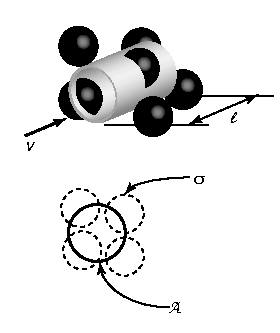
\includegraphics[width=\linewidth]{mean-free-path}
    \caption[Schematic of mean free path]{\label{f.MFP} Schematic of a particle incident on a group of scattering or absorbing particles.}
\end{marginfigure}
What is the probability of our particle making it through the cylinder unscathed? The probability of the particle hitting an obstacle is the ratio
\[
    \mathcal{P} = \frac{\textrm{total area covered by obstacles}}{\textrm{area of cylinder}}
\]
Denote the cross-sectional area of the other particles by $\sigma$. If the density of obstacles is $n$, then the number of obstacles in the cylinder is $n\times(\mathcal{A}\ell)$, and therefore the fraction of the area blocked by the obstacles is
\marginnote{We are taking $\ell$ and $\mathcal{A}$ sufficiently small that we don't have to worry about particles overlapping.}
\begin{equation}
    \mathcal{P} = \frac{n\times(\mathcal{A}\ell)\times\sigma}{\mathcal{A}} = n\sigma\ell.
\label{e.prob-MFP}
\end{equation}
The particle will suffer a collision when $\mathcal{P}\to 1$, or when
\begin{equation}\label{e.MFP}
    \ell = \frac{1}{n\sigma}.
\end{equation}
We call $\ell$ the ``mean free path'': it is the mean distance the particle travels freely before colliding.

\begin{marginfigure}[3\baselineskip]
    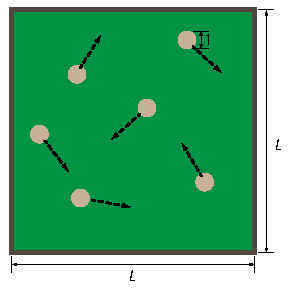
\includegraphics[width=\linewidth]{air-hockey-mfp}
    \caption[Mean free path of a hockey puck]{\label{f.MFP-2D}Schematic for Exercise~\ref{ex.MFP-2D}}
\end{marginfigure}
\begin{exercisebox}[Mean free path of a hockey puck]\label{ex.MFP-2D}
    Suppose we have a flat, slippery surface on which hockey pucks are sliding around, as shown in Fig.~\ref{f.MFP-2D}. The pucks bounce off the walls as they slide around.  Suppose there are $N$ pucks, each with unit diameter, and the table is square with sides of length $L$.  Estimate the mean free path of a puck.
\end{exercisebox}

Although we have motivated this derivation with a classical picture, the cross-section $\sigma$ is just related to the probability of an interaction and can therefore be defined for quantum mechanical systems.

\begin{exercisebox}[Mean free path for electron scattering]\label{ex.MFP}
    In the sun, free electrons scatter photons; the cross-section for this is
    \[
    \sigma_{\mathrm{Th}} = \left(\frac{8\pi}{3}\right)\left(\frac{e^2}{4\pi\epsilon_{0}\,m_e c^2}\right)^2 = \val{\sci{6.65}{-29}}{\meter^2}.
    \]
    What is the mean free path against this process for a photon at the average density of the solar interior?
\end{exercisebox}

As the ray of light traverses a small distance $\Delta s$ through some matter, the probability of a photon being absorbed is $\mathcal{P} = n\sigma\Delta s$. Thus, out of every $N$ photons, $\Delta N = N \times\mathcal{P} = N\times n\sigma\Delta s$ are absorbed. Since the intensity $I_{\nu}$ is proportional to the number of photons, the change in intensity is just
\[ \Delta I_{\nu} = -n\sigma I_{\nu}\Delta s. \]
Dividing by $\Delta s$ and taking the limit $\Delta s\to0$, we obtain an equation for the absorption of light,
\begin{equation}\label{e.absorption-microscopic}
\left.\DD{I_{\nu}}{s}\right|_{\mathrm{absorption}} = -n\sigma I_{\nu}.
\end{equation}
Rather than work with the microscopic cross-section, it is convenient to define the \newterm{absorption opacity},
\[
	\kapabs = \frac{n\sigma}{\rho},
\]
so that $\dif I_{\nu}/\dif s = -\rho\kapabs I_{\nu}$. The units of opacity are $\cm^{2}/\gram$. We use a subscript $\nu$ to indicate that the opacity is a function of frequency. In terms of the opacity, the photon mean free path is $\ell = (\rho\kapabs)^{-1}$.

\begin{exercisebox}[Attenuation of light in an absorbing medium]
A ray of light crosses a slab of absorbent material. Calculate the intensity $I_{\nu}$ as a function of distance traveled. Your expression should be in terms of $\rho$ and $\kapabs$. How far does the ray go before its intensity has dropped to $1/e$ of its original value?
\end{exercisebox}

\newthought{In addition to absorbing photons, the matter can also spontaneously emit them.} Denote the power emitted per wavelength per volume per angle by $\rho j_{\nu}$. After traveling a distance $\Delta s$ through matter with this \newterm{emissivity}, the ray will increase in intensity by $\rho j_{\nu}\Delta s$; or
\begin{equation}\label{e.emission-microscopic}
\left.\DD{I_{\nu}}{s}\right|_{\mathrm{emission}} = \rho j_{\nu}.
\end{equation}

\begin{exercisebox}[Combined absorption and emission]
Suppose a ray traverses matter that both absorbs (opacity $\kapabs$) and emits (emissivity $j_{\nu}$), so that
\[	\DD{I_{\nu}}{s} = \rho j_{\nu} - \rho\kapabs I_{\nu}. \]
Solve for $I_{\nu}(s)$, and show that as $s\to\infty$, $I_{\nu}\to j_{\nu}/\kapabs$.
\label{ex.intensity-at-large-depth}
\end{exercisebox}

\newthought{Finally, the matter can also scatter light.} This removes photons from a ray, similar to absorption, but it also adds them into a ray propagating in a different direction. 
If we assume that the direction into which the photon is scattered is random and isotropic (as is most often the case), then if the intensity in our ray is greater than the angle-average $J_{\nu}$, scattering will cause a net reduction in intensity as more photons are scattered out of the ray than are scattered into it. Conversely, if $I_{\nu} < J_{\nu}$, then more photons will be scattered into the ray than out of it. Thus, the effect of scattering can be described via
\begin{equation}\label{e.scattering-microscopic}
\left.\DD{I_{\nu}}{s}\right|_{\mathrm{scattering}} = -\rho\kapscat \left(I_{\nu} - J_{\nu}\right).
\end{equation}

\section{The equation of radiative transfer}
\label{s.equation-radiative-transfer}

Combining our expressions for absorption, emission, and scattering gives us the full expression for how the intensity changes along a ray,
\begin{equation}\label{e.transfer-equation}
\DD{I_{\nu}}{s} = -\rho\left(\kapabs + \kapscat\right) I_{\nu} + \rho j_{\nu} + \rho\kapscat J_{\nu}.
\end{equation}
This is a complicated \newterm{integrodifferential} equation: it contains both the derivative $\dif I_{\nu}/\dif s$ of the intensity as well as its integral $J_{\nu} = (4\pi)^{-1}\int I_{\nu}\,\dif\Omega$.

In general, eq.~(\ref{e.transfer-equation}) must be solved numerically; but conditions in the deep interior of the star and near the surface allow us to make simplifying approximations and to obtain a solution that gives some insight into the physics. First, let's clean up the equation: divide through by $\rho\kappa_{\nu}\equiv\rho(\kapabs + \kapscat)$,
\[
	\frac{1}{\rho\kappa_{\nu}}\dd{I_{\nu}}{s} = -I_{\nu} + \left[\frac{j_{\nu} + \kapscat J_{\nu}}{\kappa_{\nu}}\right].
\]
Next, define a new quantity, the \newterm{optical depth} $\tau_{\nu}$ via the equation
\[
	\dd{\tau_{\nu}}{s} = \rho\kappa_{\nu} = \rho(\kapabs+\kapscat),
\]
which allows us to change variables, $\dif I_{\nu}/\dif s = (\dif I_{\nu}/\dif\tau_{\nu})\cdot(\dif\tau_{\nu}/\dif s)$; and finally define the \newterm{source function} $S_{\nu}$ as the term in $\left[\cdot\right]$. Doing all that gives us the simpler-looking equation,
\[
	\DD{I_{\nu}}{\tau_{\nu}} = -I_{\nu} + S_{\nu}.
\]
This prettifying doesn't advance us any closer to the solution, but notice! The optical depth has a simple meaning:
\[
	\tau_{\nu} = \int_{0}^{s} \rho\kappa_{\nu}\,\dif s = \int_{0}^{s} n\sigma_{\nu}\,\dif s = \int_{0}^{s} \frac{\dif s}{\ell}.
\]
That is, the optical depth measures distance along the ray in units of mean free path. Said differently, if you have traveled one optical depth, then you have gone one mean free path. We also see from this equation that $I_{\nu}\to S_{\nu}$ as $\tau_{\nu}\to\infty$ (cf.\ exercise~\ref{ex.intensity-at-large-depth}).

Thus, if your object has $\tau_{\nu}\ll 1$, then photons are hardly affected by the medium and the object is nearly transparent; if, on the other hand, $\tau_{\nu} \gg 1$, then photons cannot go through the object: it is opaque, and the emission is determined by the emissivity (via the source function $S_{\nu}$) of the matter.

\begin{exercisebox}[Optical depth of the solar center]
For the electron scattering cross-section (Exercise~\ref{ex.MFP}), estimate the optical depth between the solar center and the solar photosphere.
\end{exercisebox}

\newthought{Suppose we are in a cavity in which the radiation and matter are in a steady-state}. 
The matter is not gaining or losing energy to the radiation. This requires balancing
\[ \left(\textrm{energy emitted per unit volume}\right) = \rho\int j_{\nu}\,\dif\nu\,\dif\Omega\] 
with
\[ \left(\textrm{energy absorbed per unit volume}\right) = \rho\int \kapabs I_{\nu}\,\dif\nu\,\dif\Omega,\]
so that
\begin{equation}\label{e.rad-equil}
\int_{0}^{\infty}\! \left(j_{\nu} - \kapabs J_{\nu}\right)\,\dif\nu = 0.
\end{equation}
We don't include scattering in this expression because scattering doesn't transfer energy between the radiation and the gas.

If, in addition, the matter and radiation are in thermal equilibrium, so that $J_{\nu} = B_{\nu}$, then eq.~(\ref{e.rad-equil}) implies that
\begin{equation}\label{e.detailed-balance}
\frac{j_{\nu}}{\kapabs} = B_{\nu}(T).
\end{equation}
Now $j_{\nu}$ and $\kapabs$ are properties of the matter, and do not depend on the state of the radiation field. Hence, equation~(\ref{e.detailed-balance}) must hold whenever the matter is in equilibrium, \emph{regardless of the state of the radiation field}.

\section{Radiative diffusion}

We can now examine how heat transport works in the deep interior of a star. First, we need to adjust our coordinates. In equation~(\ref{e.transfer-equation}), the coordinate $s$ is distance along a ray; but we are considering many different rays. We shall therefore use radial distance $r$ as a coordinate, and measure the optical depth it: $\dif\tau_{\nu} = \rho\kappa_{\nu}\,\dif r$. 
Since $\dif r = \mu\,\dif s$, where $\mu=\cos\theta$ is the cosine between $\dif s$ and $\dif r$ (Fig.~\ref{f.dr-ds-relation}), the equation of transfer becomes
\begin{equation}
\mu\DD{I_{\nu}}{r} = -\rho\kappa_{\nu}\left(I_{\nu} - S_{\nu}\right).
\end{equation}
\begin{marginfigure}
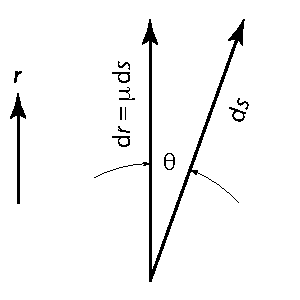
\includegraphics[width=\linewidth]{dr-ds-relation}
\caption[Coordinates for radiative transport equation]{\label{f.dr-ds-relation} Schematic of the coordinate system used for solving the radiative transport equation.}
\end{marginfigure}

\newthought{Let's examine the typical scales of terms in the radiative transfer equation, for conditions in the deep solar interior.} We'll start with eq.~(\ref{e.transfer-equation}), and indicate some expected scales:
\[
\underbrace{\mu\DD{I_{\nu}}{r}}_{\sim I_{\nu}/\Rsun} = -\underbrace{\rho\kappa_{\nu} I_{\nu}}_{\sim I_{\nu}/\ell}  +\rho\kappa_{\nu} S_{\nu}.
\]
If we are far from the surface of the star, then we should expect the intensity to change over lengthscales comparable to $\Rsun$. Of course, it won't be exactly this, but---as we'll show---the exact value doesn't matter so long as $|\dif I_{\nu}/\dif s|$ is in the ballpark of $I_{\nu}/\Rsun$. Notice the enormous disparity in scales:
\[
	\frac{|\dif I_{\nu}/\dif r|}{\rho\kappa_{\nu}I_{\nu}} \sim \frac{\ell}{\Rsun};
\]
the left-hand side is smaller than the terms on the right by the ratio of the mean free path to the solar radius. This implies that conditions are nearly homogeneous. They are also isotropic, so that $I_{\nu} = J_{\nu}$. We expect that collisions are fast enough so that the matter is in thermal equilibrium and $j_{\nu} = \kapabs B_{\nu}$. We also know from exercise~\ref{ex.intensity-at-large-depth} that $I_{\nu} \to j_{\nu}/\kapabs = B_{\nu}$.

We can't have $I_{\nu} = B_{\nu}$ exactly, however, since in that case there is no net flux! We'll treat the intensity as being thermal plus a perturbation:
\[ I_{\nu} = B_{\nu} + I_{\nu}^{(1)}, \]
where the superscript ``(1)'' indicates that this is a small correction. Inserting this expansion into eq.~(\ref{e.transfer-equation}) and keeping only the lowest-order terms on each side gives
\begin{equation}\label{e.perturbation-radiative-transfer}
I_{\nu}^{(1)} = -\mu\DD{B_{\nu}}{\tau_{\nu}}.
\end{equation}
$B_{\nu}$ depends on the temperature $T$, so $\dif B_{\nu}/\dif\tau_{\nu} = \dif B_{\nu}/\dif T \cdot \dif T/\dif \tau_{\nu}$. To get the flux, multiply eq.~(\ref{e.perturbation-radiative-transfer}) by $\mu$ and integrate over angles:
\[ F_{\nu} = \int\mu I_{\nu}^{(1)}\,\dif\Omega = -\int \mu^{2}\DD{B_{\nu}}{T}\,\DD{T}{\tau_{\nu}}\,\dif \Omega = -\frac{4\pi}{3} \DD{B_{\nu}}{T}\,\DD{T}{\tau_{\nu}}. \]
We can switch back to the radial coordinate:
\begin{equation}\label{e.specific-radiative-transport}
	F_{\nu} = -\frac{4\pi}{3}\left[\frac{1}{\rho\kappa_{\nu}}\dd{B_{\nu}}{T}\right]\DD{T}{r}.
\end{equation}
The term in $\left[\cdot\right]$ controls which frequencies are most responsible for energy transport.

\begin{exercisebox}[Transport by frequency]
\label{ex.radiative-transfer}
Let's examine the term $\left[\cdot\right]$ in eq.~(\ref{e.specific-radiative-transport}) more closely. Fig.~\ref{f.planck} shows $B_{\nu}$ and $\dif B_{\nu}/\dif T$ (top panel) and a hypothetical $\kappa_{\nu}$ (middle). Sketch $F_{\nu}$ on the bottom panel.  For which frequencies is it maximum?
\end{exercisebox}

\begin{marginfigure}
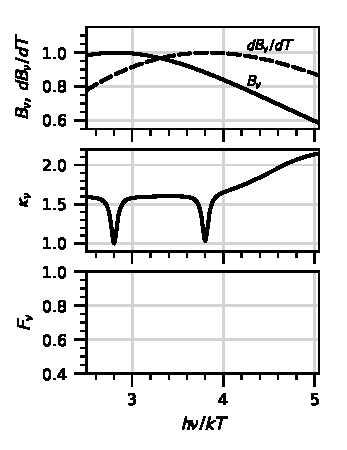
\includegraphics[width=\linewidth]{radiative-transfer-exercise}
\caption{\label{f.planck} The specific flux for a hypothetical opacity}
\end{marginfigure}

To get the total flux, we integrate $F_{\nu}$ over all frequencies. 
\begin{eqnarray*}
	F = \int_{0}^{\infty}F_{\nu}\,\dif\nu &=& -\frac{4\pi}{3} \left[\int_{0}^{\infty} \frac{1}{\rho\kappa_{\nu}}\dd{B_{\nu}}{T}\right]\DD{T}{r}\\
	&\equiv& -\frac{4\pi}{3}\frac{1}{\rho\kappa_{\mathrm{R}}}\dd{}{T}\left[\int_{0}^{\infty}B_{\nu}\,\dif\nu\right]\DD{T}{r}.
\end{eqnarray*}
Here we've defined the \newterm{Rosseland mean} of the opacity:
\begin{equation}\label{e.rosseland-opacity}
	\frac{1}{\kappa_{\mathrm{R}}} = \left(\int_{0}^{\infty} \dd{B_{\nu}}{T}\,\dif\nu\right)^{-1}\int_{0}^{\infty} \frac{1}{\kappa_{\nu}}\dd{B_{\nu}}{T}\,\dif\nu.
\end{equation}
This is done to put the equation in more familiar terms. Since (cf.\ eq.~[\ref{e.bolometric-thermal-flux}]) $\int B_{\nu}\,\dif\nu = \sigmaSB T^{4}/\pi = c a T^{4}/4\pi$, we can write the equation for the flux as
\begin{equation}
	F = -\frac{1}{3}\frac{c}{\rho\kappa_{\mathrm{R}}}\DD{}{r}aT^{4}.
\label{e.radiative-transfer}
\end{equation}
Equation (\ref{e.radiative-transfer}) is known as the equation for radiative diffusion, for reasons that will become apparent in the next section.

If we multiply the flux by the surface area of a shell in the star we obtain the luminosity $L = 4\pi r^{2} F$; we can therefore recast eq.~(\ref{e.radiative-transfer}) into an equation for the thermal gradient:
\begin{equation}
    \label{e.gradient-temperature}
    \DD{T}{r} = -\frac{3\rho\kappa_{R}}{4acT^3}\frac{L(r)}{4\pi r^2}.
\end{equation}

\begin{exercisebox}[Radiative transfer equation]
\label{ex.radiative-transfer-diffusion}
Let's dissect eq.~(\ref{e.radiative-transfer}) to see how it sets the luminosity.  
\begin{enumerate}
\item\label{p.F-L}
To keep the algebra simple, assume that $F$ is constant throughout the star and that $aT^{4}$ is linear in $r$---that is, $aT^{4} = aT_{c}^{4}(1-r/R)$.  Since $F$ is constant, you can express it in terms of the luminosity at the surface $L$.  Use this to transform eq.~(\ref{e.radiative-transfer}) into an expression for $L$ in terms of $R$ and $T_{c}$ (along with $\rho$, $\kappa_{\mathrm{R}}$, and $c$).

\item\label{p.L-tau}
Write the luminosity as $L = E_{\gamma}/\tau$, where $E_{\gamma}$ is the total radiative energy of the star, and $\tau$ some as-yet-undetermined \emph{diffusion timescale}.  Give an estimate of $E_{\gamma}$ in terms of the mean temperature $T$ and the radius $R$ of the star.

\item\label{p.tau}
Finally, assume that the photon mean free path $\ell = (\rho\kappa_{\mathrm{R}})^{-1}$ is constant.  Substitute the results from parts \ref{p.F-L} and \ref{p.L-tau} into equation~(\ref{e.radiative-transfer}).  After simplifying, you should end up with a simple expression for $\tau$ in terms of $c$, $R$, and $\ell$.  For Thomson scattering, what is $\tau$ (express in years)?
\end{enumerate}
\end{exercisebox}

\section{Diffusion}\label{s.diffusion}

In the presence of scattering or absorption, the photons crossing the face can travel one mean free path $\ell$. Imagine a small cube with sides of length $\ell$ and filled with photons. The total radiant energy in the cube is $\Delta E$. In a time $\Delta t = \ell/c$, all of the photons will leave this cube. The total luminosity is $\Delta E/\Delta t = c\Delta E/\ell$. If everything is isotropic, then the flux out of any one face is $1/6$ of the luminosity, divided by the area of that face:
\[
	F = \frac{1}{6\ell^{2}}\frac{c\Delta E}{\ell} = \frac{1}{6}c U,
\]
where $U = E/\ell^{3}$ is the radiative energy density. 

Now place two of these cubes against one another, with their common face located at position $x$. The energy density of the two cubes need not be the same; the energy density of the left cube is $U(x-\ell)$ and of the right cube is $U(x+\ell)$ (see Fig.~\ref{f.diffusive-flux}). The net flux traveling in the $x$-direction through the common face is then
\[
	F = {\color{blue}\frac{1}{6} c U(x-\ell)} - {\color{red}\frac{1}{6} c U(x+\ell)} \approx -\frac{1}{3}c\ell \DDx{U}.
\]
This is an expression for a \newterm{diffusive flux}. Although we gave a heuristic explanation, the formula is in general true:
\begin{eqnarray}
\nonumber
(\textrm{flux of something}) &=& -\frac{1}{3}\times(\textrm{speed of carriers})\times(\textrm{MFP of carriers})\\
&&\times \grad(\textrm{density of something})
\label{e.diffusive-flux}
\end{eqnarray}
For radiation, the ``something'' is ``radiative energy'' and the carriers are photons.
\begin{marginfigure}[-12\baselineskip]
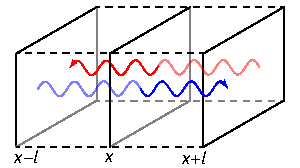
\includegraphics[width=\linewidth]{diffusive-flux}
\caption[Transport along a gradient]{\label{f.diffusive-flux} Illustration of net flux crossing a face between regions with slightly different energy densities.}
\end{marginfigure}

\begin{exercisebox}[Rosseland weighting]
Compare this crude diffusion model,
\[
	F = -\frac{1}{3}c\ell\DD{U}{r},
\]
with eq.~(\ref{e.radiative-transfer}). Using the results of exercise~\ref{ex.radiative-transfer}, give a succinct description for why the effective mean free path $\ell = 1/(\rho\kappa_{\mathrm{R}})$ is computed using a weighting function $\partial B_{\nu}/\partial T$.
\end{exercisebox}

\begin{marginfigure}
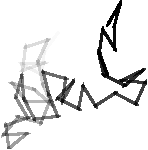
\includegraphics[width=\linewidth]{random-walk-schematic}
\caption[Schematic of a random walk]{\label{f.random-walk-schematic}Schematic of a random walk of 50 steps.}
\end{marginfigure}
\newthought{As an alternate take on our estimation, let's model the transport as a photon that is randomly walking throughout the interior.}
The photon moves at speed $c$, but it can only go one mean free path $\ell$ before being absorbed or scattered, at which point it is sent off in a random direction.\marginnote{To keep things simple, we'll imagine that after absorption the atom immediately emits an identical photon in a random direction.} The path of the photon will therefore look something like that in Fig.~\ref{f.random-walk-schematic}.

We will just do our calculation for motion along a diameter, with the photon starting at the center. At each hop, the photon either goes left or right with equal probability. On average, the photon doesn't go anywhere; but after enough hops, there is some probability for the photon to reach the edge of the star and escape. Figure~\ref{f.random-walk} shows the distribution of positions for walks of length $n = 10, 30, 100, 300$ steps, with each step having length 1.0. Suppose the edge of the star is at $x=\pm 10$ (red dotted lines).  Although the average position is at $x=0$, for $n \gtrsim 100$ steps, there is a reasonable probability of the photon escaping.
\begin{figure}[htbp]
\forceversofloat
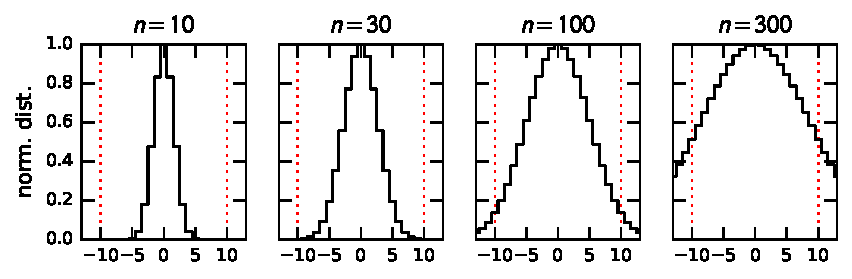
\includegraphics[width=\linewidth]{random-walk}
\caption[Distribution of positions in a random walk]{\label{f.random-walk} Distribution of positions after $n$ steps in a random walk.}
\end{figure}

To make this into a workable model, let us first recall the basic features of a random walk. It is described by a binomial distribution: after $n$ steps, the probability that $m$ of them were to the right is
\begin{equation}\label{e.binomial}
    \binom{n}{m}{p} = \frac{n!}{m!(n-m)!} p^{m}(1-p)^{n-m}.
\end{equation}
Here $p$ is the probability of any single step being to the right.
The mean and root variance of $m$ are
\begin{eqnarray}
	\mean{m} &=& np \label{e.mean-binomial} \\
	\left[\mean{\left(m-\mean{m}\right)^{2}}\right]^{1/2} &=& \left[np(1-p)\right]^{1/2}. \label{e.var-binomial}
\end{eqnarray}
We can use these to estimate the diffusion timescale $\tau$.

\begin{exercisebox}[Radiative diffusion as a random walk]
\label{ex.random-walk-diffusion}
\begin{enumerate}
\item
Show from equation~(\ref{e.mean-binomial}) that the mean distance traveled by the photon after $n$ steps is $\langle d\rangle = \ell(2np-n)$, so for $p=1/2$, $\langle d\rangle = 0$.

\item\label{p.straight-line-steps}
If all the steps were in the same direction, how many steps would be needed to reach the edge, at a a distance $R$ from the center? Assume all steps have the same length $\ell$.

\item
We want the distribution of steps (cf.\ Fig.~\ref{f.random-walk}) to be wide enough to reach the edge. Set the root variance---a measure of the width of the probability distribution---equal to the number of steps found in part \ref{p.straight-line-steps} and use equation~(\ref{e.var-binomial}),
	\[
		\left[\mean{\left(m-\mean{m}\right)^{2}}\right]^{1/2} = 
			\left[n_{\mathrm{edge}}p(1-p)\right]^{1/2},
	\]
	to find $n_{\mathrm{edge}}$ in terms of $R$ and $\ell$.

\item
What is the \emph{total} distance traveled by the photon after $n_{\mathrm{edge}}$ steps? If the photon traveled at speed $c$, how long did it take? Compare your answer with that for part~\ref{p.tau} of exercise~\ref{ex.radiative-transfer-diffusion}.

\end{enumerate}
\end{exercisebox}

\section{The photosphere}

We are now ready to investigate heat transport near the edge, where the optical depth $\tau_{\nu} \lesssim 1$ and photons begin to freely escape. We can no longer use the approximation of radiative diffusion, because conditions in the star are now changing over distances of a mean free path. Let's return to equation~(\ref{e.transfer-equation}) for radiative transport:
\[
	\DD{I_{\nu}}{s} = -\rho\left(\kapabs + \kapscat\right) I_{\nu} + \rho j_{\nu} + \rho\kapscat J_{\nu}.
\]
In general, this is difficult to solve: for some frequencies, the atmosphere will be nearly transparent, while for other frequencies it is quite opaque. Rather than develop the numerical machinery to solve the equation, we shall adopt a few simple approximations (indicated by highlighted bold text in the margins) that will allow us to obtain an approximate solution for the temperature of the stellar atmosphere.

\marginnote[\baselineskip]{\colorbox{yellow}{\textbf{Opacities are gray}}}First, we assume that the opacity is gray---that is, independent of frequency. This is unphysical, but the solutions for temperature and pressure will have the correct overall behavior. Because the opacity is gray, we shall drop the ``$\nu$'' subscript in $\kappa$ and $\tau$.

\begin{exercisebox}[Gray emissivity?]
Does matter with a gray opacity in thermal equilibrium also have a gray emissivity $j_{\nu}$?
\end{exercisebox}

We next define a coordinate system. Since we are in a thin layer near the edge of the star, we will adopt planar coordinates, with $z$ being the altitude above some point. We'll pick $z=0$ to be a point deep enough in the star that $I_{\nu}\approx B_{\nu}$. Then we define the optical depth as
\begin{equation}\label{e.optical-depth-planar}
	\tau = \int_{z}^{\infty} \rho\left(\kappa^{\mathrm{abs}}+\kappa^{\mathrm{sca}}\right)\,\dif z ;
\end{equation}
differentiating this expression gives
\[
	\DD{\tau}{z} = -\rho\left(\kappa^{\mathrm{abs}}+\kappa^{\mathrm{sca}}\right).
\]
Note the ``$-$'': in these coordinates, as $z$ gets larger, $\tau$ gets smaller.

We may rewrite the equation (\ref{e.hydrostatic-equilibrium-g}) of hydrostatic balance as
\begin{eqnarray}
	-\rho g = \DD{P}{z} &=& \DD{P}{\tau}\DD{\tau}{z} = -\rho\kappa\DD{P}{\tau},\nonumber\\
	\DD{P}{\tau} &=& \frac{g}{\kappa}.
\label{e.P-tau}
\end{eqnarray}
Since we are in a thin layer, we can take the gravitational acceleration $g$ as being approximately constant. By integrating hydrostatic equilibrium from where $\tau = 0, P = 0$ to where $\tau = 1$, we can get an approximate value of the photospheric pressure,
\[
	P_{\mathrm{ph}} = \int_{0}^{P_{\mathrm{ph}}}\,\dif P = \int_{0}^{1}\frac{g}{\kappa}\,\dif\tau \approx \frac{g}{\kappa}.
\]
\begin{quote}
\emph{The surface gravity sets the pressure at the \textbf{photosphere}, the location where the optical depth is of order unity and where photons can escape from the star.}
\end{quote}

\begin{exercisebox}[Photospheric pressure]
Suppose you observe a star that has a 10\% larger mass and 10\% larger radius than the sun. All else being equal, how does the pressure at the photosphere of this star compare to that of the sun?
\end{exercisebox}

\marginnote[\baselineskip]{\colorbox{yellow}{\textbf{Atmosphere is in steady-state LTE}}}
For our second approximation, we assume that the matter is in \newterm{local thermal equilibrium} (LTE). This means there is a well-defined temperature at each depth. Furthermore, the emissivity is related to the absorption opacity,
\[
	j_{\nu} = \kappa^{\mathrm{abs}}B_{\nu}.
\]
Note that this does \emph{not} imply anything about the radiation field. We can now take the radiative transfer equation (\ref{e.transfer-equation}) and substitue our definition of optical depth (eq.~[\ref{e.optical-depth-planar}]) to obtain
\begin{equation}\label{e.transfer-gray}
	\mu\DD{I_{\nu}}{\tau} = I_{\nu} - S_{\nu}.
\end{equation}
Here
\[
	S_{\nu} = \frac{j_{\nu} + \kappa^{\mathrm{sca}} J_{\nu}}{\kappa}
	= \frac{\kappa^{\mathrm{abs}} B_{\nu} + \kappa^{\mathrm{sca}} J_{\nu}}{\kappa}.
\]
If, in addition, the matter is in steady-state, then the rate at which energy is absorbed from the radiation field, $\int\kappa^{\mathrm{abs}}I_{\nu}\,\dif\nu\,\dif\Omega$, must equal the rate at which energy is emitted, $\int j_{\nu}\,\dif\nu\,\dif\Omega$. Since we are in LTE,
\[
	\int \left(j_{\nu} - \kappa^{\mathrm{abs}}I_{\nu}\right)\,\dif\nu\,\dif\Omega
	= 4\pi\kappa^{\mathrm{abs}}\int\left(B_{\nu} - J_{\nu}\right)\,\dif\nu = 0.
\]
Since $J = \int J_{\nu}\,\dif\nu = \int B_{\nu}\,\dif\nu = B$, it follows that $S = \int S_{\nu}\,\dif\nu = B$ as well:
\begin{quote}
\emph{For a gray atmosphere in steady-state, local thermal equilibrium, the integrated source function and mean intensity equal the Planck value:}
\[ S(\tau) = J(\tau) = B(\tau), \]
\end{quote}
Note that this does \emph{not} imply that $I_{\nu}=B_{\nu}$ or $J_{\nu}=B_{\nu}$.

We still have the problem that eq.~(\ref{e.transfer-gray}) includes both the derivative and integral of $I_{\nu}$. To get around this, we are going to expand $I_{\nu}$ in Legendre polynomials,
\[
	I_{\nu}(\tau,\mu) = I_{\nu,0}(\tau)\Pl{0}(\mu) + I_{\nu,1}(\tau)\Pl{1}(\mu) + I_{\nu,2}(\tau)\Pl{2}(\mu) + \ldots
\]
and then only include the first two terms, $\Pl{0}(\mu) = 1, \Pl{1} = \mu$. Thus, $I_{\nu}$ is \emph{linear} in $\mu$: $I_{\nu} = I_{\nu,0}(\tau) + I_{\nu,1}(\tau)\mu$. 
\marginnote{\colorbox{yellow}{\textbf{Intensity is linear in $\mu$}}}

In terms of this expansion, the angle-averaged specific intensity is
\[
	J_{\nu}(\tau) = \frac{1}{4\pi}\int I_{\nu}\,\dif\mu\,\dif\phi = I_{\nu,0}(\tau),
\]
and hence the specific energy density is $U_{\nu} = 4\pi/c\cdot J_{\nu} = 4\pi/c\cdot I_{\nu,0}$. The specific flux is
\[
	F_{\nu}(\tau) = \int \mu I_{\nu}\,\dif\mu\,\dif\phi = \frac{4\pi}{3} I_{\nu,1}(\tau).
\]
We can therefore write the intensity as
\begin{equation}
\label{e.intensity-expanded}
I_{\nu}(\tau) = J_{\nu}(\tau) + \frac{3\mu}{4\pi} F_{\nu}(\tau) = \frac{c}{4\pi}U_{\nu}(\tau) + \frac{3\mu}{4\pi} F_{\nu}(\tau).
\end{equation}

\begin{sidebar}[Expansion in Legendre polynomials]
\label{sb.intensity-decomposition}
You may recall from electrostatics that we can decompose the field from a set of charges into a sum of moments: dipole, quadrupole, and so on. The basis functions for this are the Legendre polynomials $\Pl{n}(\cos\theta)$, defined by the expansion
\[
	\frac{1}{\sqrt{1 - 2\mu z + z^{2}}} \equiv \sum_{n=0}^{\infty}\Pl{n}(\mu)z^{n},
\]
for $-1<\mu<1,\;|z| < 1$. The first four polynomials are
\begin{eqnarray*}
	\Pl{0}(\mu) = 1 &\quad& \Pl{2}(\mu) = \frac{1}{2}(3\mu^{2}-1)\\
	\Pl{1}(\mu) = \mu &\quad& \Pl{3}(\mu) = \frac{1}{2}(5\mu^{3}-3\mu),
\end{eqnarray*}
and the first eight Legendre polynomials are plotted below.

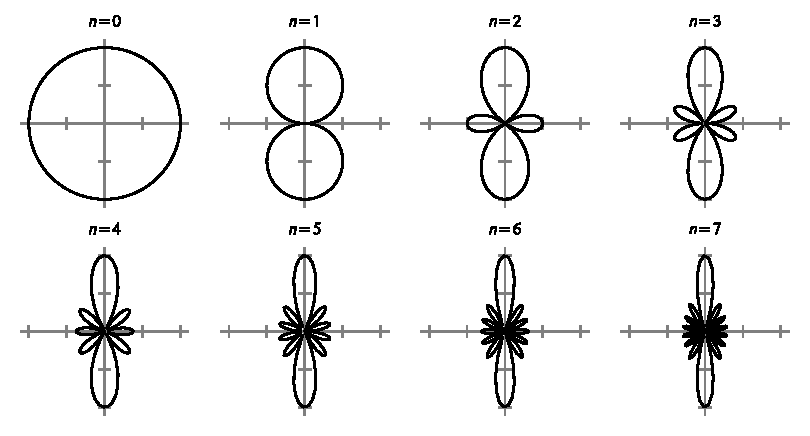
\includegraphics{legendre}

\noindent As $n$ increases, the angular variations become finer.

The Legendre polynomials are \emph{orthogonal} in the following sense:
\begin{equation}\label{e.orthogonal}
\int_{-1}^{1}\Pl{n}(\mu)\Pl{m}(\mu)\dif \mu = \left\{
\begin{array}{lr}
	0 &  m\neq n\\
	\frac{2}{2n+1} & m=n
\end{array}\right..
\end{equation}
As a result of this orthogonality, we can decompose the radiative intensity into multipoles:
\begin{equation}\label{e.decomposition}
	I = \sum_{n=0}^{\infty} I_{n} \Pl{n}(\mu).
\end{equation}

\begin{exercisebox}[Odd-even powers of $\mu$]
\label{e.symmetry-powers-mu}
Use eq.~(\ref{e.orthogonal}) to show that $(4\pi)^{-1}\int I\,\dif\Omega = I_{0}$ and $\int \mu I\,\dif\Omega = (4\pi/3)I_{1}$, for $I = I_{0} + I_{1}\mu$.
\end{exercisebox}

\end{sidebar}

Insert the expansion (\ref{e.intensity-expanded}) into the radiative transfer equation (\ref{e.transfer-gray}) and integrate over all angles and frequencies. Since $\tau$ is gray, we can pull the derivative out from the integral,
\begin{eqnarray*}
	\DD{}{\tau}\int \mu I_{\nu}\,\dif\nu\,\dif\Omega &=& \int I_{\nu}\,\dif\nu\,\dif\Omega - \frac{\kappa^{\mathrm{abs}}}{\kappa}\int B_{\nu}\,\dif\nu\,\dif\Omega - \frac{\kappa^{\mathrm{sca}}}{\kappa} \int J_{\nu}\,\dif\nu\,\dif\Omega\\
	\DD{}{\tau}\int F_{\nu}\,\dif\nu &=& \frac{4\pi}{\kappa}\left[
		(\kappa^{\mathrm{abs}}+\kappa^{\mathrm{sca}})\int J_{\nu}\,\dif\nu
		- \kappa^{\mathrm{abs}}\int B_{\nu}\,\dif\nu
		- \kappa^{\mathrm{sca}}\int J_{\nu}\,\dif\nu\right]\\
	\DD{F}{\tau} &=& 4\pi\frac{\kappa^{\mathrm{abs}}}{\kappa}\int\left(J_{\nu}-B_{\nu}\right) = 0.
\end{eqnarray*}
Here we used $\kappa = \kappa^{\mathrm{abs}}+\kappa^{\mathrm{sca}}$ to simplify the right-hand side.

\begin{quote}
\emph{For a steady-state gray atmosphere in local thermal equilibrium, the total flux $F = \int F_{\nu}\,\dif\nu$ is constant.}
\end{quote}
The radiative energy is just passing through. Since the flux at $\tau=0$, outside the star, is $F = \sigmaSB\,\Teff^{4}$, we can substitute that value in our expression for the intensity,
\begin{equation}
\label{e.Inu-expansion}
	I(\mu,\tau) = \frac{c}{4\pi} U(\tau) + \frac{3\mu}{4\pi}\sigmaSB\Teff^{4}.
\end{equation}
To solve for $U(\tau)$, multiply eq.~(\ref{e.transfer-gray}) by $\mu$ and integrate over all angles and frequencies:
\begin{eqnarray}
	\DD{}{\tau}\int\mu^{2}I_{\nu}\,\dif\Omega\,\dif\nu &=& \int\mu I_{\nu}\,\dif\Omega\,\dif\nu
		- \int \mu S_{\nu}\,\dif\Omega\,\dif\nu\nonumber\\
	\frac{c}{4\pi}\DD{}{\tau} \int \mu^{2}U\,\dif\Omega 
		+ \frac{3}{4\pi}\sigmaSB\Teff^{4}\int\mu^{3}\,\dif\Omega &=& F - \int \mu S\,\dif\Omega\nonumber\\
	\frac{c}{3}\DD{U}{\tau} &=& \sigmaSB\Teff^{4}
\label{e.ODE-U}
\end{eqnarray}
In going from the first to the second line we have used eq.~(\ref{e.Inu-expansion}). In going from the second to the third line, the integrals of $\mu^{3}$ and $\mu S$ vanish because $S$ is independent of angle and $\int_{-1}^{1} \mu\,\dif\mu = \int_{-1}^{1}\mu^{3}\,\dif\mu = 0$. 

Equation~(\ref{e.ODE-U}) is a first-order ODE, which upon integration yields
\begin{equation}\label{e.energy-density-Eddington}
	U(\tau) = \frac{3}{c}F(\tau + \tau_{0}),
\end{equation}
where $\tau_{0}$ is an integration constant. Our intensity is thus
\[
	I(\mu,\tau) = \frac{3}{4\pi}\sigmaSB\Teff^{4}\left(\tau + \tau_{0} + \mu\right).
\]
To fix the integration constant $\tau_{0}$, let's go to where $\tau=0$. Here all of the radiation must be outward-bound. Hence if we integrate $\mu I(\mu,\tau=0)$ over $0\le\mu\le 1$, we should recover the flux:
\[
	\sigmaSB\Teff^{4} = \int_{0}^{2\pi}\int_{0}^{1} \mu I(\mu,\tau=0)\,\dif\mu\,\dif\phi
	= \frac{3}{4}\sigmaSB\Teff^{4}\left(\tau_{0} + \frac{2}{3}\right),
\]
which fixes $\tau_{0} = 2/3$.

To finish this, we note that $J = B$ since we are in steady-state local thermal equilibrium. The radiative energy density is thus $U = (4\pi/c) J = (4\pi/c)B = 4\sigmaSB/c T^{4}$. Substituting this into eq.~(\ref{e.energy-density-Eddington}) then yields
\begin{equation}\label{e.T-tau}
T^{4} = \frac{3}{4}\Teff^{4}\left(\tau + \frac{2}{3}\right).
\end{equation}
This equation, along with eq.~(\ref{e.P-tau}), determines the structure of the stellar atmosphere.

\begin{sidebar}[Decomposition of intensity into moments]
\label{sb.intensity-moments}
It is often useful to describe the intensity in terms of \newterm{moments}. A moment is simply an angle-weighted average of the radiative intensity, where the weight is a power of $\mu$. For example, to take the zeroth-order moment, we multiply $I_{\nu}$ by $\mu^{0}=1$, integrate over all angles, and divide by $4\pi$. This is just the average intensity $J_{\nu} = (4\pi)^{-1}\int I_{\nu}\,\dif\Omega$. To take the first-order moment $H_{\nu}$, we use a weight $\mu^{1}$:
\[
	H_{\nu} = \frac{1}{4\pi}\int_{0}^{2\pi}\int_{-1}^{1}\mu I_{\nu}\,\dif\mu\,\dif\phi.
\]
To take the second-order moment $K_{\nu}$, we use a weight $\mu^{2}$:
\[
	K_{\nu} = \frac{1}{4\pi}\int_{0}^{2\pi}\int_{-1}^{1}\mu^{2} I_{\nu}\,\dif\mu\,\dif\phi.
\]
The first three moments have physically interpretable meanings: the specific radiative energy density, flux, and pressure are $U_{\nu} = (4\pi/c)J_{\nu}$, $F_{\nu} = 4\pi H_{\nu}$, and $P_{\nu} = (4\pi/c) K_{\nu}$, respectively.

By taking moments of the radiative-transfer equation~(\ref{e.transfer-gray}), we reduce the complicated integro-differential equation into a simpler ordinary differential equation. This comes at a cost, however; because the left-hand side contains $\mu\dif/\dif\tau$, the left hand side will have a higher-order moment than the right-hand side. By multiplying eq.~(\ref{e.transfer-gray}) by successively higher powers of $\mu$ and integrating, we will generate an infinite series of ODE's for successively higher moments of $I_{\nu}$.
The trick is to adopt a \newterm{closure relation} that truncates this series. The classic scheme, due to Eddington, is to take $K = J/3$.
The Eddington closure scheme is equivalent to expanding the radiative intensity to terms linear in $\mu$.

\begin{exercisebox}[The Eddington closure scheme]
Show that if we approximate the intensity as $I_{\nu}(\mu,\tau) = I_{\nu,0}(\tau) + \mu I_{\nu,1}(\tau)$ (cf.\ eq.~[\ref{e.intensity-expanded}]), then $K_{\nu} = J_{\nu}/3$ identically.
\end{exercisebox}
\end{sidebar}

\begin{exercisebox}[Anisotropy of the intensity]
Deep in the star, we expect the radiation to be nearly isotropic, while it becomes outward-bound as $\tau\to 0$. Let's investigate this. We'll measure the anisotropy of the radiation field using the first two moments of the intensity (Box~\ref{sb.intensity-moments}).
\begin{enumerate}
\item
Demonstrate that $H_{\nu}/J_{\nu} = 0$ if the radiation is isotropic.

\item
Next, suppose the radiation is completely anisotropic: all the photons are headed along precisely the same direction $\mu = 1$. We describe this mathematically as
\begin{equation}
I_{\nu}(\mu) = a_{\nu} \delta(\mu - 1),
\end{equation}
where $\delta(x)$ is the \newterm{Dirac delta function} (see Box~\ref{sb.delta-function}).
Show that $H_{\nu}/J_{\nu} = 1$ for this case.

\item
Now compute $H(\tau)/J(\tau)$ for our gray atmosphere.What is the degree of anisotropy at $\tau = 0$? at $\tau=2/3$? at $\tau = 10$?
\end{enumerate}
\end{exercisebox}

\begin{sidebar}[The Dirac delta function]
\label{sb.delta-function}
The Dirac delta function $\delta(x)$ has the following properties: $\delta(x) = 0, \forall x \neq 0$; and
\[
\int_{-\epsilon}^{\epsilon} \delta(x)\,\dif x = 1.
\]
From this definition, one can show that
\[
	\int f(x) \delta(x-a)\,\dif x = f(a),
\]
where the integral is over any domain containing $x = a$.
\end{sidebar}

